%!TEX root = ../docu.tex
\section{Konzept}

\subsection{Grundkonzept}

Das folgende Kapitel erläutert die Kozeptionierung der Anwendung, welche im späteren Verlauf implementiert wird. Hierbei handelt es sich um eine Applikation die hauptsächlich für das Abspielen von Hörbüchern im Audioformat MP3 genutzt werden soll. Die Applikation ist so ausgelegt, das alle Funktionen einfach erreichbar und bedienbar sind.

Die Applikation soll dem Benutzer ermöglichen Hörbücher abzuspielen, welche er vorher auf sein mobiles Endgerät abgelegt hat. Hierfür muss die Applikation eine Einstellungsmöglichkeit beinhalten. Über diese Einstellung muss der Benutzer den Speicherort wählen und festlegen. Über diesen Einstellungsparameter ist es der Anwendung nun möglich alle Audiodateien aufzulisten und abzuspielen. Die Auflistung filtert alle nicht abspielbaren Daten und ermöglicht des Weiteren in Unterordnen zu navigieren. Ein Element der Liste stellt dabei entweder eine Audiodatei oder ein Unterordner dar. 

\begin{figure}[h!t]
\begin{center}
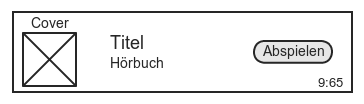
\includegraphics[scale=0.8]{images/listitem}
\caption{Mockup für ein Listenelement}
\label{mocklistel}
\end{center}
\end{figure}

Die Abbildung \ref{mocklistel} beschreibt ein solches Element. Es enthält das Cover des Hörbuches sowie den Titel und die genau Abspielzeit. Aus dieser Auflistung heraus werden alle Audiodateien abgespielt die sich im aktuellen Verzeichnis befinden. Eine Schnittstelle zur Übertragung der Informationen zur Player-Komponente realisiert diese Funktion. Diese Komponente ist für das eigentliche Abspielen zuständig. Sie empfängt die Anweisung zum Abspielen der Audiodatei und spielt dieses Datei ab.

\begin{figure}[ht]
\begin{minipage}[b]{0.45\linewidth}
\centering
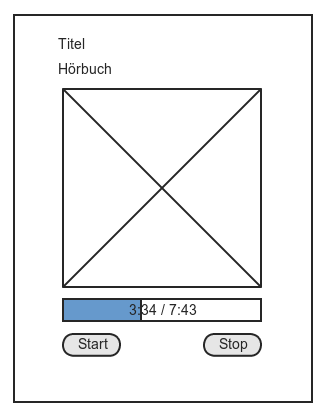
\includegraphics[width=\textwidth]{images/playerkomp}
\caption{Konzept des Players}
\label{playerkomp}
\end{minipage}
\hspace{0.5cm}
\begin{minipage}[b]{0.45\linewidth}
\centering
\fbox{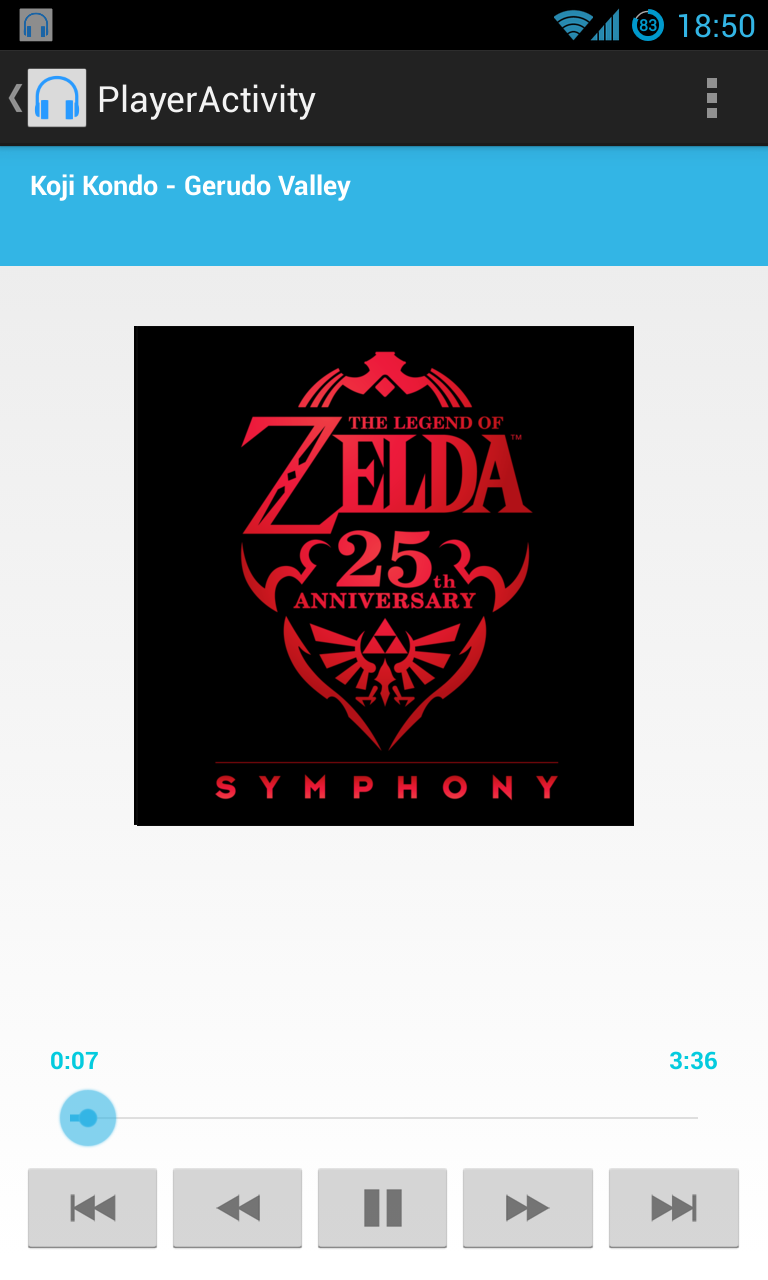
\includegraphics[width=\textwidth]{images/player_unframed}}
\caption{Player-Implementierung}
\label{player}
\end{minipage}
\end{figure}

Die Player-Komponente wie in Abbildung \ref{playerkomp} als Mockup und in Abbildung \ref{player} als realer Screenshot dargestellt, ermöglicht das Abspielen zu steuern. Dies beinhaltet das Stoppen, Pausieren und andere Funktionen. Des Weiteren ist Erkennbarkeit welche Audiodatei abgespielt wird. Eine Vorschrittanzeige lässt erkennen, wie viel von der Audiodatei bisher abgespielt wird sowie die Gesamtlänge der Audiodatei.

\begin{figure}
\begin{center}
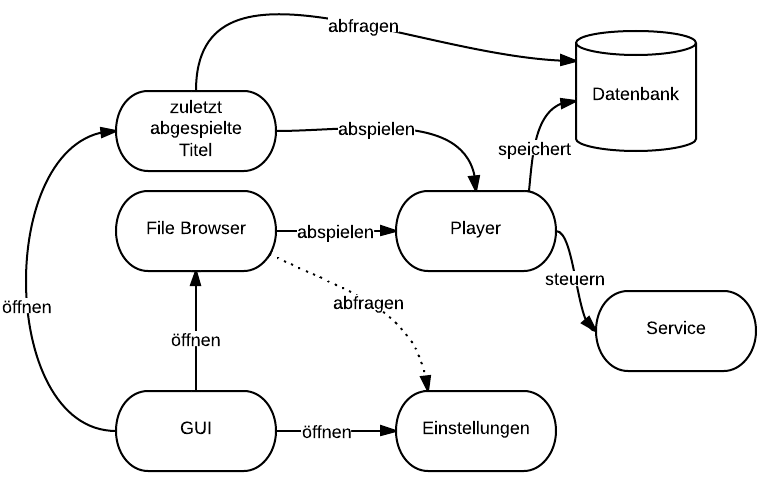
\includegraphics[scale=0.6]{images/konzept}
\caption{Schematische Darstellung der Anwendung}
\label{konzept}
\end{center}
\end{figure}

Wird die Anwendung beendet wird die Wiedergebe abgebrochen. Sie ist in der Lage Abbrüche der Wiedergabe zu erkennen und diese zu speichern. Der Benutzer hat dann die Möglichkeit, die Wiedergabe an diesen Punkten fortzusetzen.

Die Eingabe erfolgt durch ein übliches Touchscreen-Display und ist darauf optimiert. Hierzu gehört klare und einfache Programmstrukturen sowie ausreichend große Flächen für Bedienelemente und Steuerung von Programmfunktionen. Die gesamte Programmstruktur ist so aufgebaut, dass eine Weiterentwicklung und Implementierung neuer Funktionen möglich ist.